\documentclass{standalone}
\usepackage{tikz}
\usepackage{circuitikz}

\begin{document}
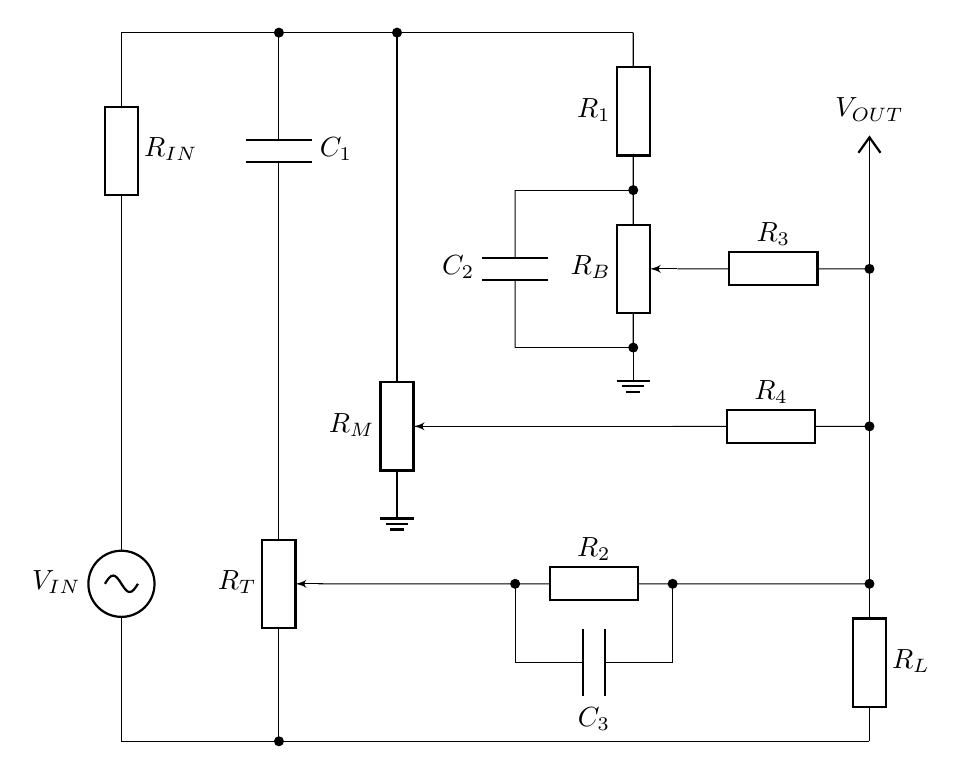
\begin{tikzpicture}
	\draw (2, 5) to[sinusoidal voltage source, l_=$V_{IN}$] (2, 1);

	\draw (2, 10) to[european resistor, l=$R_{IN}$] (2, 7);
	\draw (8.5, 8) to[european resistor, l=$R_1$] (8.5, 10);
	\draw (11.5, 3) to[european resistor, l_=$R_2$] (4.5, 3);
	\draw (9.06, 7) to[european resistor, l=$R_3$] (11.5, 7);
	\draw (9, 5) to[european resistor, l=$R_4$] (11.5, 5);
	\draw (11.5, 3) to[european resistor, l=$R_L$] (11.5, 1);

	\draw (4, 10) to[capacitor, l=$C_1$] (4, 7);
	\draw (7, 8) to[capacitor, l_=$C_2$] (7, 6);
	\draw (7, 2) to[capacitor, l_=$C_3$] (9, 2);

	\draw (8.5, 8) to[european potentiometer, l_=$R_B$] (8.5, 6);
	\draw (5.5, 5.75) to[european potentiometer, l_=$R_M$] (5.5, 4.25);
	\draw (4, 5) to[european potentiometer, l_=$R_T$] (4, 1);

	\draw (2, 10) -- (8.5, 10);
	\draw (11.5, 1) -- (2, 1);
	\draw (2, 5) -- (2, 7);
	\draw (4, 5) -- (4, 7);
	\draw (5.5, 5.75) -- (5.5, 10);
	\draw (9, 5) -| (6.06, 5);
	\draw (7, 2) -- (7, 3);
	\draw (7, 8) -- (8.5, 8);
	\draw (7, 6) -- (8.5, 6);
	\draw (9, 2) -- (9, 3);
	\draw (11.5, 8.25) -- (11.5, 6.75);
	\draw (11.5, 3) -- (11.5, 7);

	\node[ground] at (5.5, 4.25) {};
	\node[ground] at (8.5, 6) {};
	\node[vcc] at (11.5, 8.25) {$V_{OUT}$};
	\node[circ] at (11.5, 3) {};
	\node[circ] at (11.5, 5) {};
	\node[circ] at (11.5, 7) {};
	\node[circ] at (4, 1) {};
	\node[circ] at (4, 10) {};
	\node[circ] at (5.5, 10) {};
	\node[circ] at (7, 3) {};
	\node[circ] at (8.5, 6) {};
	\node[circ] at (8.5, 8) {};
	\node[circ] at (9, 3) {};

\end{tikzpicture}
\end{document}